
%(BEGIN_QUESTION)
% Copyright 2011, Tony R. Kuphaldt, released under the Creative Commons Attribution License (v 1.0)
% This means you may do almost anything with this work of mine, so long as you give me proper credit

This magnetic flowmeter is used to measure the flow of water through a pipe at a powdered milk processing plant.  As you can see, the pipe size is reduced at the flowmeter, expanding to regular size upstream and downstream of the meter:

$$\epsfxsize=5in \includegraphics[width=15.5cm]{i03426x01.eps}$$

Explain why the piping has been sized like this.

\underbar{file i03426}
%(END_QUESTION)





%(BEGIN_ANSWER)

Possible answers include:

\begin{itemize}
\item{} Decreased cost (smaller meter)
\item{} Increased velocity (greater millivoltage generated for better resolution/accuracy)
\item{} Compensate for upstream piping disturbances by accelerating fluid more
\item{} Helps ensure meter tube remains full of liquid
\item{} Increased velocity to help scrub electrodes of microbial growth
\end{itemize}

Grading will be proportional to the number of reasons given.  For example, if a student gives three reasons for this flowmeter installation and only two of them are good, deduct 3 points; if a student gives two reasons and only one is good, deduct 5 points.

%(END_ANSWER)





%(BEGIN_NOTES)

{\bf This question is intended for exams only and not worksheets!}.

%(END_NOTES)

